\section{A learned portfolio of complete reduction strategies}
\label{sec:portfolio}
The preceding comparisons show that the useful decision depends on both the denominator structure and the target powers. A seed region that suffices for one batch can leave another batch unreduced, while expanding every seed limit can generate equations that the calculation does not need. We therefore train a model to choose a complete calculation from several strategies before Kira generates the equations. This choice includes the previous workflow as a candidate, so the new policy can retain that workflow when its measured cost is lower.

\subsection{What the model chooses}
For a target batch, let $r_0$ be the largest sum of positive indices, $s_0$ the largest total numerator power, and $d_0$ the largest number of extra denominator powers, or dots. Kira uses limits of this kind to define the seed region~\cite{Kira3}. Our earlier complete-cost policy chooses among seven regions or equation settings, as described in Appendix~\ref{sec:adaptive}. A development comparison reveals a useful additional choice: increase $s_0$ by one while leaving the positive-index and dot limits unchanged. This selective expansion can supply missing identities without the cost of increasing all three limits.

The final portfolio contains five choices: the earlier cost policy with one or two workers, selective numerator-rank expansion with one or two workers, and the previous workflow from Appendix~\ref{app:thread-policy}. A worker carries out tasks in Kira's existing parallel symbolic solver~\cite{KiraOriginal}. The previous workflow combines its existing graph, seed, and worker choices; its parameters remain fixed in this comparison. Each choice uses the same exact preprocessing and a supplied master basis. The three- and four-loop bubble boxes have no trained policy in the previous workflow, so its control uses the documented native fallback. We retain Kira's native row elimination because the learned row model has not reduced complete time reliably.

Each attempt must express every target in the prescribed basis. If it cannot do so, the calculation retries with native seeds and then an expanded seed region. We skip a repeated attempt when its effective seed bounds, ordering, and equation filter are identical to those already tried. The model does not predict reduction coefficients. It predicts the relative time of these complete strategies, including checks, failed attempts, and recovery. Appendix~\ref{app:portfolio} defines the model inputs, objective, guard, and exact recovery procedure.

\subsection{Training and independent tests}
We fit 30 candidate predictors using 47 training batches and select the predictor, fixed control, and decision threshold using 26 separate validation batches. The candidates include regression trees, random forests, and extremely randomized trees~\cite{CART1984,Breiman2001Forest,Geurts2006ExtraTrees}. Their twenty inputs describe the graph structure, target powers, numerator ranks, number of targets, and distribution of dots. They contain no reference coefficients or measured test times. The recorded label calculations take 1858.3 seconds, and fitting takes 2.621 seconds. These costs occur before deployment.

For each graph, validation also selects the fastest fixed portfolio choice. The model replaces this choice only if it reduces summed validation time by at least two percent and gives a saving in both validation repetitions. This rule enables target-dependent portfolio predictions for planar double box, three-loop two-point ladder, nonplanar box, sunrise. All enabled outer predictors are single regression trees. A retained portfolio choice can itself contain an earlier learned policy; therefore the fixed-portfolio control isolates the added outer decision, rather than removing all earlier learned decisions. Requests outside the recorded graph structures and feature ranges use native settings.

The reserved test uses rational kinematic profile $h=306$ and symbolic targets with a dot position absent from the earlier symbolic training and validation sets. The earlier reserved profiles do not enter fitting or selection. The completed comparison contains 26 batches from nine known graph structures through four loops, with one to three targets per batch. Appendix~\ref{app:portfolio} specifies the targets and reference checks. These tests change kinematics and target positions within known structures; some rational target patterns recur across profiles. They do not test transfer to arbitrary new graphs or larger target batches.

Every method receives the same two-core allocation and an 8\,GiB memory allowance. The native control and earlier cost-policy control use one Kira worker. The previous workflow, fixed portfolio, and selected portfolio can use one or two workers according to their chosen strategy. We rotate method order and repeat each method three times, with a fresh Kira process and temporary files for every attempt. Complete time includes prediction, preparation, exact algebra, coefficient checks, cleanup, and recovery. Model imports, initial model loading, reference construction, and basis discovery are separate. No coefficient cache supplies the test answers.

\subsection{Complete-time results}
Table~\ref{tab:portfolio} sums the three-run median times of the individual batches. The selected portfolio takes 85.497 seconds, compared with 108.029 seconds for native choices and 95.382 seconds for the previous workflow in the same improved executable. These results correspond to 20.9\% less time than native choices and 10.4\% less time than the previous workflow. The earlier cost policy takes 102.561 seconds on these same inputs. The graph-specific fixed portfolio takes 86.809 seconds, so the added portfolio decision gives 1.5\% less time relative to this stronger control. Figure~\ref{fig:portfolio-controls} shows where these differences occur.

Summing every timed repetition gives 19.4\% less time than native choices, 9.4\% less time than the previous workflow, and 0.4\% more time than the fixed portfolio. The small difference from the fixed portfolio changes sign between the two summaries. These measurements establish no stable aggregate saving from the added outer prediction. The practical improvement over the previous workflow includes the revised candidate strategies and worker choices, which also benefit the fixed portfolio.

\begin{table}[!htbp]\centering\small
\caption{Complete reduction times in seconds. Each row sums batch medians from matched tests with common exact preprocessing. ``Fixed'' selects a portfolio choice per graph using validation only.}
\label{tab:portfolio}
\begin{tabular}{@{}lrrrr@{}}\toprule
Graph & Native & Previous & Fixed & Selected\\\midrule
Three-loop bubble box & 2.280 & 2.300 & 2.274 & 2.388\\
Four-loop bubble box & 32.420 & 29.726 & 28.981 & 29.129\\
Planar double box & 9.478 & 8.226 & 8.179 & 7.406\\
Three-loop two-point ladder & 23.326 & 17.584 & 14.314 & 14.108\\
Nonplanar box & 28.380 & 25.414 & 20.793 & 20.236\\
Virtuality box & 2.585 & 2.756 & 2.763 & 2.608\\
Pentagon & 3.895 & 3.922 & 4.072 & 3.966\\
Sunrise & 1.941 & 1.677 & 1.661 & 1.770\\
Three-loop vacuum & 3.724 & 3.777 & 3.772 & 3.886\\
\midrule Total & 108.029 & 95.382 & 86.809 & 85.497\\\bottomrule
\end{tabular}\end{table}

All 390 timed reductions and 26 further applications reproduce the reference coefficients exactly. The applications receive only the prescribed master basis before reduction; the comparison with reference coefficients follows execution. The selected portfolio requires 3 recovery attempts across the timed tests. Its median outer decision time is 0.575 milliseconds. The CPU-time totals are 115.370 seconds for native choices and 114.666 seconds for the selected portfolio. Reporting both wall and CPU time separates elapsed-time savings from changes in CPU use, as shown in Figure~\ref{fig:portfolio-totals}. Every planned batch completes both reference calculations.

The dotted three-loop two-point ladder illustrates the change in the equation system. Native choices use seed limits $(10,0,2)$, then $(11,1,3)$, while the selected portfolio uses $(10,1,2)$, in the order $(r,s,d_{\rm dots})$. Summing the reported generated-equation counts across all attempts gives medians of 287,558 equations for native choices and 94,380 for the selected portfolio. Their complete times are 14.637 and 7.345 seconds. This count measures equation generation; symbolic simplification can require different work per equation. The CPU-time comparison also accounts for the effect of worker count.

The application also avoids loading the previous workflow until a selected strategy requires it. On the dotted sunrise batch, three rotated comparisons of a new application instance give median request times of 3.258 seconds with immediate loading and 0.727 seconds with deferred loading. These times include construction, one reduction, an exact coefficient check, and closure, while common Python imports remain outside the timer. All six requests choose the same strategy and return the same exact coefficients. This separate interface saving applies when the request does not need the previous workflow. A request that first selects that workflow pays its loading cost within the application time. The repeated portfolio timings above already keep the models loaded, so they receive no additional saving from this change.

\begin{figure}[tbp]\centering
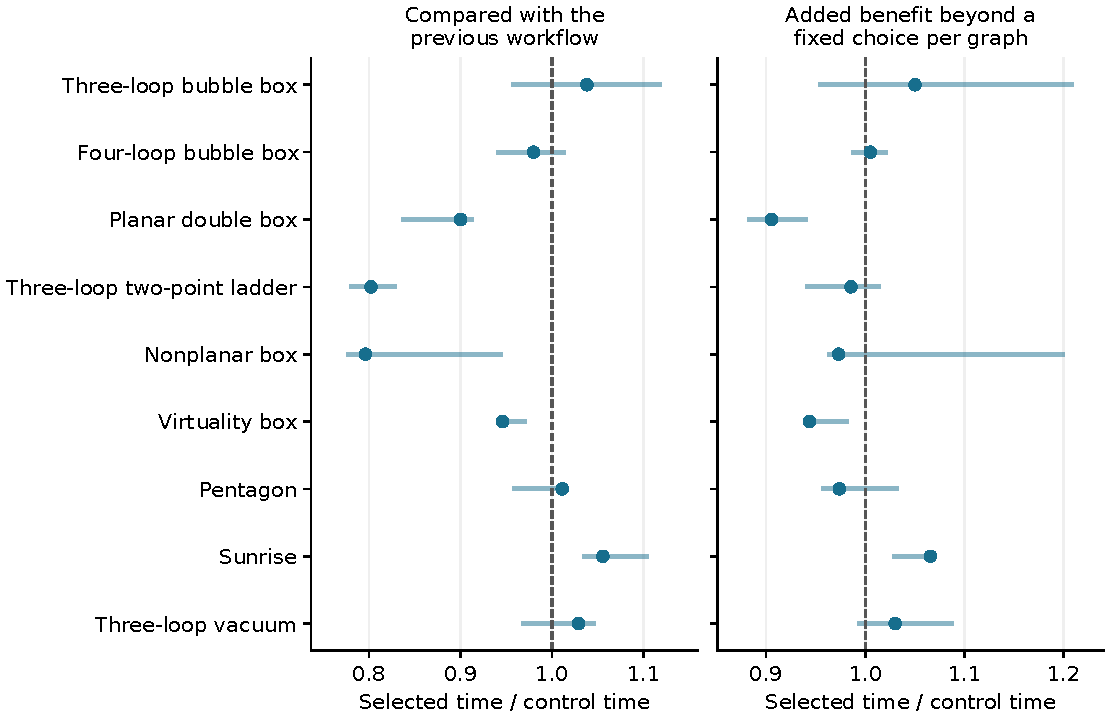
\includegraphics[width=\linewidth]{paper_figures/portfolio_controls.pdf}
\caption{Selected-portfolio time relative to the previous workflow and the graph-specific fixed portfolio. Points divide sums of batch median times. Horizontal segments show the range of the three corresponding repetition totals; they are descriptive ranges, not confidence intervals. Values below one indicate a saving.}
\label{fig:portfolio-controls}\end{figure}

\begin{figure}[tbp]\centering
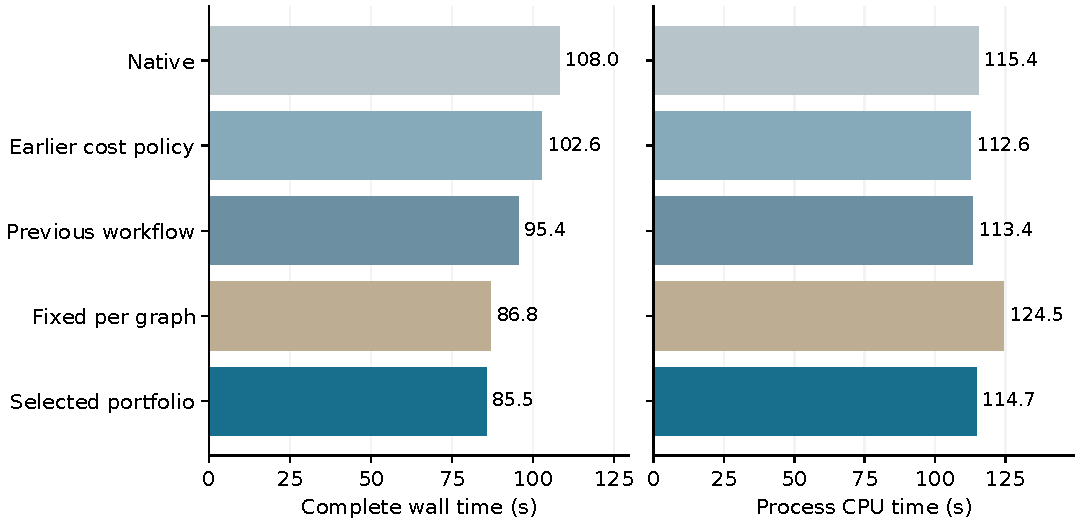
\includegraphics[width=\linewidth]{paper_figures/portfolio_totals.pdf}
\caption{Complete wall time and recorded process CPU time for the same reserved batches. The five methods share exact preprocessing and a two-core allocation. CPU time counts the main driver, Kira child processes, and the timed part of the previous-workflow service. Its message conversion lies outside that service's CPU counter but remains in complete wall time. Initial loading lies outside the repeated timings.}
\label{fig:portfolio-totals}\end{figure}

\subsection{Separating the exact implementation changes}
The portfolio tests use two exact improvements in every method. We index the sector files that exist instead of searching for absent files, while retaining their original processing order. We also simplify the criterion for zero sectors by setting Feynman parameters absent from all declared top sectors to zero before forming that criterion. The complete parametric polynomials remain available for the other operations. Appendix~\ref{app:adaptive} proves why this projection preserves the criterion in the declared sector domain, following the parametric treatment of zero sectors~\cite{Lee2014LiteRed}.

Separate matched tests enable these changes in sequence for connected bubble boxes. For the 3-loop batch, the complete time changes from 6.087 to 2.939 seconds with the first study's validated policy, an overall factor of 2.07. The 4-loop previous-preparation control does not complete after 1190.6 seconds across its bounded attempts. Further repetitions of this failed control are omitted, while the remaining settings are completed. The fully improved calculation takes 28.666 seconds, but the incomplete control supplies no measured overall speedup factor. With file indexing already enabled, projection changes its complete time from 98.408 to 28.197 seconds, a factor of 3.49. These comparisons include exact implementation changes and therefore do not measure an isolated ML gain. Figure~\ref{fig:adaptive-integration} and Table~\ref{tab:adaptive-integration} preserve the intermediate controls in the earlier cost study. The common-preprocessing comparison in Table~\ref{tab:portfolio} measures the subsequent portfolio choices separately.

The measurements support the selected strategies in the stated domain. Timing differences can remain when two methods choose the same strategy, and the three repetitions do not establish a significant gain for every graph. General higher-loop scattering, arbitrary symbolic kinematics, automatic discovery of a minimal master basis, and globally optimal elimination paths remain outside the demonstrated scope.
